\documentclass[review]{elsarticle}

\usepackage{lineno,hyperref}
\modulolinenumbers[5]

\journal{Advances in Water Resources}

%%%%%%%%%%%%%%%%%%%%%%%
%% Elsevier bibliography styles
%%%%%%%%%%%%%%%%%%%%%%%
%% To change the style, put a % in front of the second line of the current style and
%% remove the % from the second line of the style you would like to use.
%%%%%%%%%%%%%%%%%%%%%%%

%% Numbered
%\bibliographystyle{model1-num-names}

%% Numbered without titles
%\bibliographystyle{model1a-num-names}

%% Harvard
%\bibliographystyle{model2-names.bst}\biboptions{authoryear}

%% Vancouver numbered
%\usepackage{numcompress}\bibliographystyle{model3-num-names}

%% Vancouver name/year
%\usepackage{numcompress}\bibliographystyle{model4-names}\biboptions{authoryear}

%% APA style
%\bibliographystyle{model5-names}\biboptions{authoryear}

%% AMA style
%\usepackage{numcompress}\bibliographystyle{model6-num-names}

%% `Elsevier LaTeX' style
\bibliographystyle{elsarticle-num}
%%%%%%%%%%%%%%%%%%%%%%%

\begin{document}

\begin{frontmatter}

\title{ Segmentation and Classification of Porous Media X-ray Images using Convolutional Neural Networks}


%% Group authors per affiliation:
\author{Efim Lavrukhin}

\author[mysecondaryaddress]{Gerke Kirill\corref{mycorrespondingauthor}}
\cortext[Gerke]{Corresponding author}
\ead{cheshik@.com}

%% or include affiliations in footnotes:
\author[mymainaddress,mysecondaryaddress]{Sizonenko Timothey}

\author[mymainaddress,mysecondaryaddress]{Korost Dmitry}

\author[tritaryaddress]{Tarasenko Sergey}

\address[mymainaddress]{Moscow, Russia}
\address[mysecondaryaddress]{Some Street}
\address[tritaryaddress]{Independent Researcher}

\begin{abstract}
Write abtract of the paper
\end{abstract}

\begin{keyword}
porous medium \sep image processing \sep convolutional neural network \sep image segmentation \sep segmentation networks
\end{keyword}

\end{frontmatter}

\linenumbers

\section{Introduction}

\section{Background and previous works}

\section{Methodology}
\subsection{Image processing applications for porous medium analysis}
\subsection{Convolutional neural networks for segmentation: breif review and benefits}
\subsection{Classifiers}

\section{Experiments}

\subsection{Porous medium specs}

\subsection{Our model}

Key features of U-net architecture:
\begin{itemize}
	\item Fully-convolutional 
	\item Encoder-decoder acrchitecture with skip-connections
	\item Max pooling layres for comression in encoder part
	\item Transposed convolutional layers + concatenation with skip-connected encoder feature map for uncompression in decoder part
	\item Convolutional layers only with 3x3 filters
\end{itemize}

\begin{figure}[h]
	\center{
		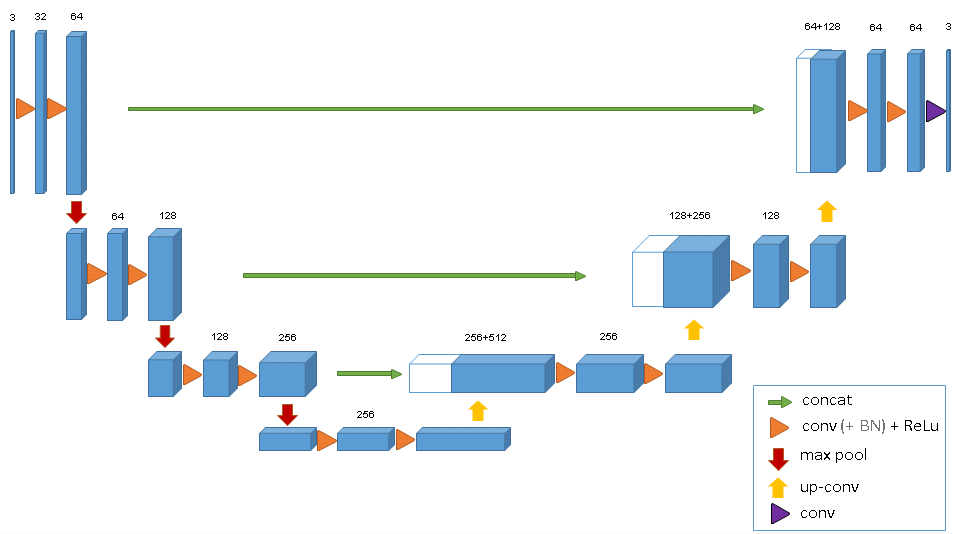
\includegraphics[width=1\linewidth]
			{data/Unet_architecture.png}
	}
	\caption{Unet architecture: ToDo}
	\label{Unet:architecture}
\end{figure}

We used Unet architecture  with some small features: 
\begin{itemize}
	\item Number of conv filters is multiplied by 32(insted of 64 in original article)
	\item Padding to conv filters, so network do not compress output
	\item ELU activation functions
	
\end{itemize}

\subsection{Learning process}

We using 2-d image patches for model training. We chose patch size $=64$ and minibatch size $=32$, so out model get 
float 4-d tensor of size $32 \times 1 \times 64 \times 64$.
Pixel intensivity scaled to $[-0.5, 0.5]$ interval.
Model returns probabilities for each pixel, model output has 
size $4096 \times 2$(besause on the top of model used 
1-d softmax activation), that output could be reshaped to size $32 \times 2 \times 64 \times 64$.

In each epoch only $\frac{1}{5}$ of minibatches used for training, because our trainig set is large enougth and full processing will be
very time expensive. We do not use data augmentation for the same reason.
    
We used combination of cross-entropy and smoothed IOU as loss function:
\begin{equation}{\label{Loss}}
	L(x, y) = \frac{1}{N} 
		\sum \limits_{i = 1}^{N} 
		\sum \limits_{x, y \in I_{i}, M_{i}} 
		\frac{1}{W H} \Bigl( 
		y \log p(x) 
		+ \alpha \log 
		\frac{p(x) y + \varepsilon}{p(x) + y - p(x)y + \varepsilon}
		\Bigr)
\end{equation}
with $\varepsilon=10^{-5}$.

We used Adam optimizer with initial learning rate $=10^{-3}$ and 
multiplicative learning rate decay to $10^{-5}$ until final epoch.

\subsection{Experimantal set-up}

We handle image stacks in folowing way:
\begin{enumerate}
 	\item Split each 2-d image to minimal overlapping patches,
 	feed patches to our model and get probabilities for each pixel.
 	\item Patches with probabilities binarized with some threshold 			so we get 
 	segmentation mask that contains our class labels.
 	\item 2-d mask for source image is assembled from probabilities 		patches. 
\end{enumerate}
\begin{figure}[h]
	\center{
		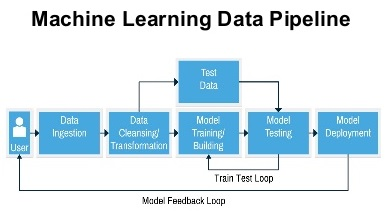
\includegraphics[width=1\linewidth]
			{data/data_pipeline.jpg}
	}
	\caption{Trainig pipeline: ToDo}
	\label{Unet:training}
\end{figure}


We choose 3 rock types: carbonate, soil and sanstone. We have 
4 carbonate, 4 soil and 3 sandstone stacks. We choose one of stacks from each category as trained(carbonate 1, soil 1 and sandstone 1).
Then we train 3 models on each trained stack independenlty, 3 models on each pair of trained stacks and one model on both trained stacks.
As result we have 7 models to compare.

Each models have training set  with equal number of images, so 
models that trained on single stack type get full stack as input,
models that trained on two stack types get a half of eash stack as input and model that trained on all three stack types get third part
of stacks.    

We measure different metrics(logloss, IOU, accuracy, precision, recall, PR-AUC) with diffent thresholds on each of 11 stacks.


\section{Results}

In out experiments we used 6 metrics:
accuracy measures number of right predicted pixels,
precision measures number of right predicted positive class pixels relative to number of total emount of predicted positive pixels,s
logloss is a metric, that takes into account predicted propapiblities of each pixels, recall measures number of right predicted positive class pixels relative to number of total emount 
of true positive pixels, PR-AUC is area under precission-recall curve, IOU is relation between intersection of predicted and true positive labels and union of predicted and true positive labels.
We measure 6 metrics for each pair of used model and predicted stack. 

\subsection{Segmentation threshold}

At first, we need to determine probabilty threshold in order to get binary segmentation. It seems to be a dificult task, but we traced the dependence of our metric from thresholds and found wide large plateau on this graphics. So we could take any threshold and get same quality of segmentation.

\begin{figure}[h]
	\center{
		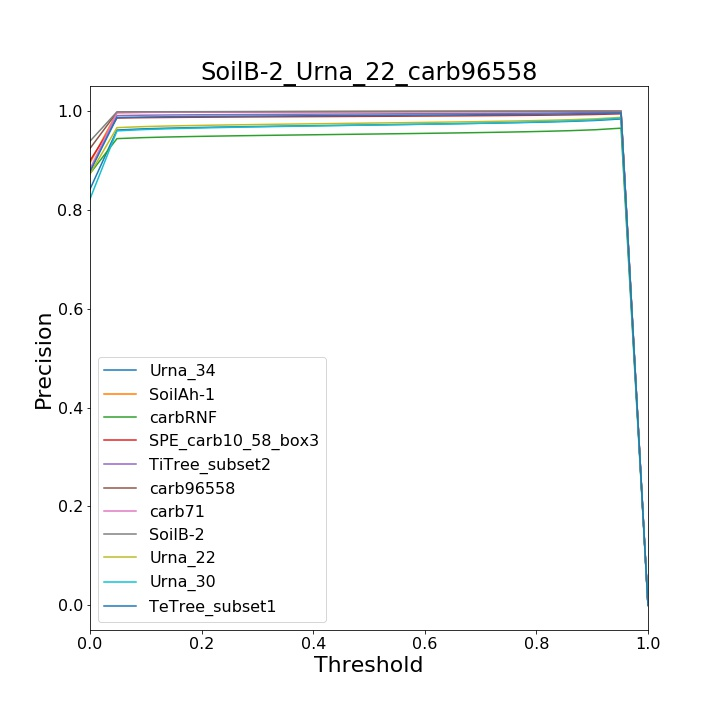
\includegraphics[width=1\linewidth]
			{data/results/SoilB-2_Urna_22_carb96558/precision.jpg}
	}
	\caption{Dependency of metrics from threshold}
	\label{Results:threshold_precision}
\end{figure}

\begin{figure}[h]
	\center{
		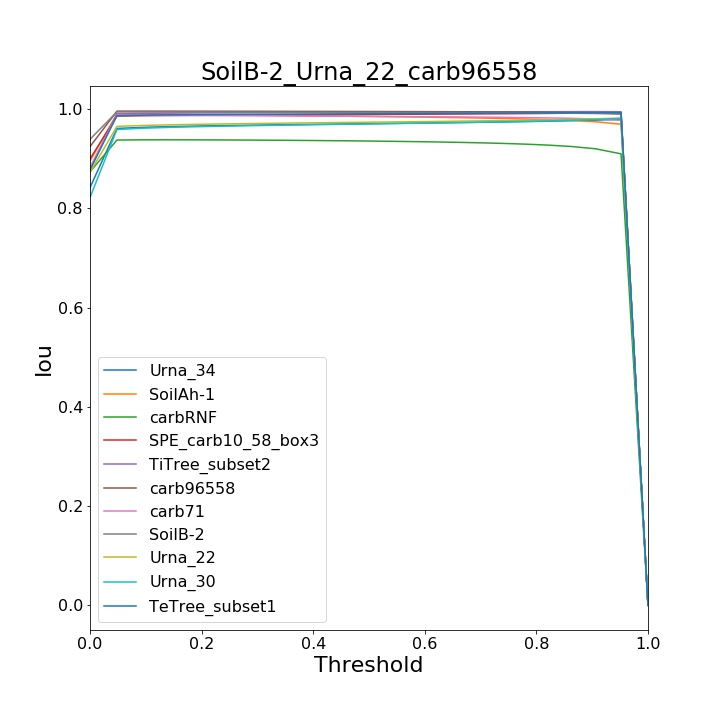
\includegraphics[width=1\linewidth]
			{data/results/SoilB-2_Urna_22_carb96558/iou.jpg}
	}
	\caption{Dependency of metrics from threshold}
	\label{Results:threshold_iou}
\end{figure}


\subsection{Visual segmentation results}

In this section we show visual results of segmentation. 
As we can see, our model is uncertaion about border pixels, so 
amount of false-negative error is much more that amount of false-positive error(false-negative pixels are colored in blue, false-positive in red).
Also there is another artifacts: some models classify bright solid clusters as pores(because there is no such clusters in trainig set of that models).

\begin{figure}[h]
	\center{
		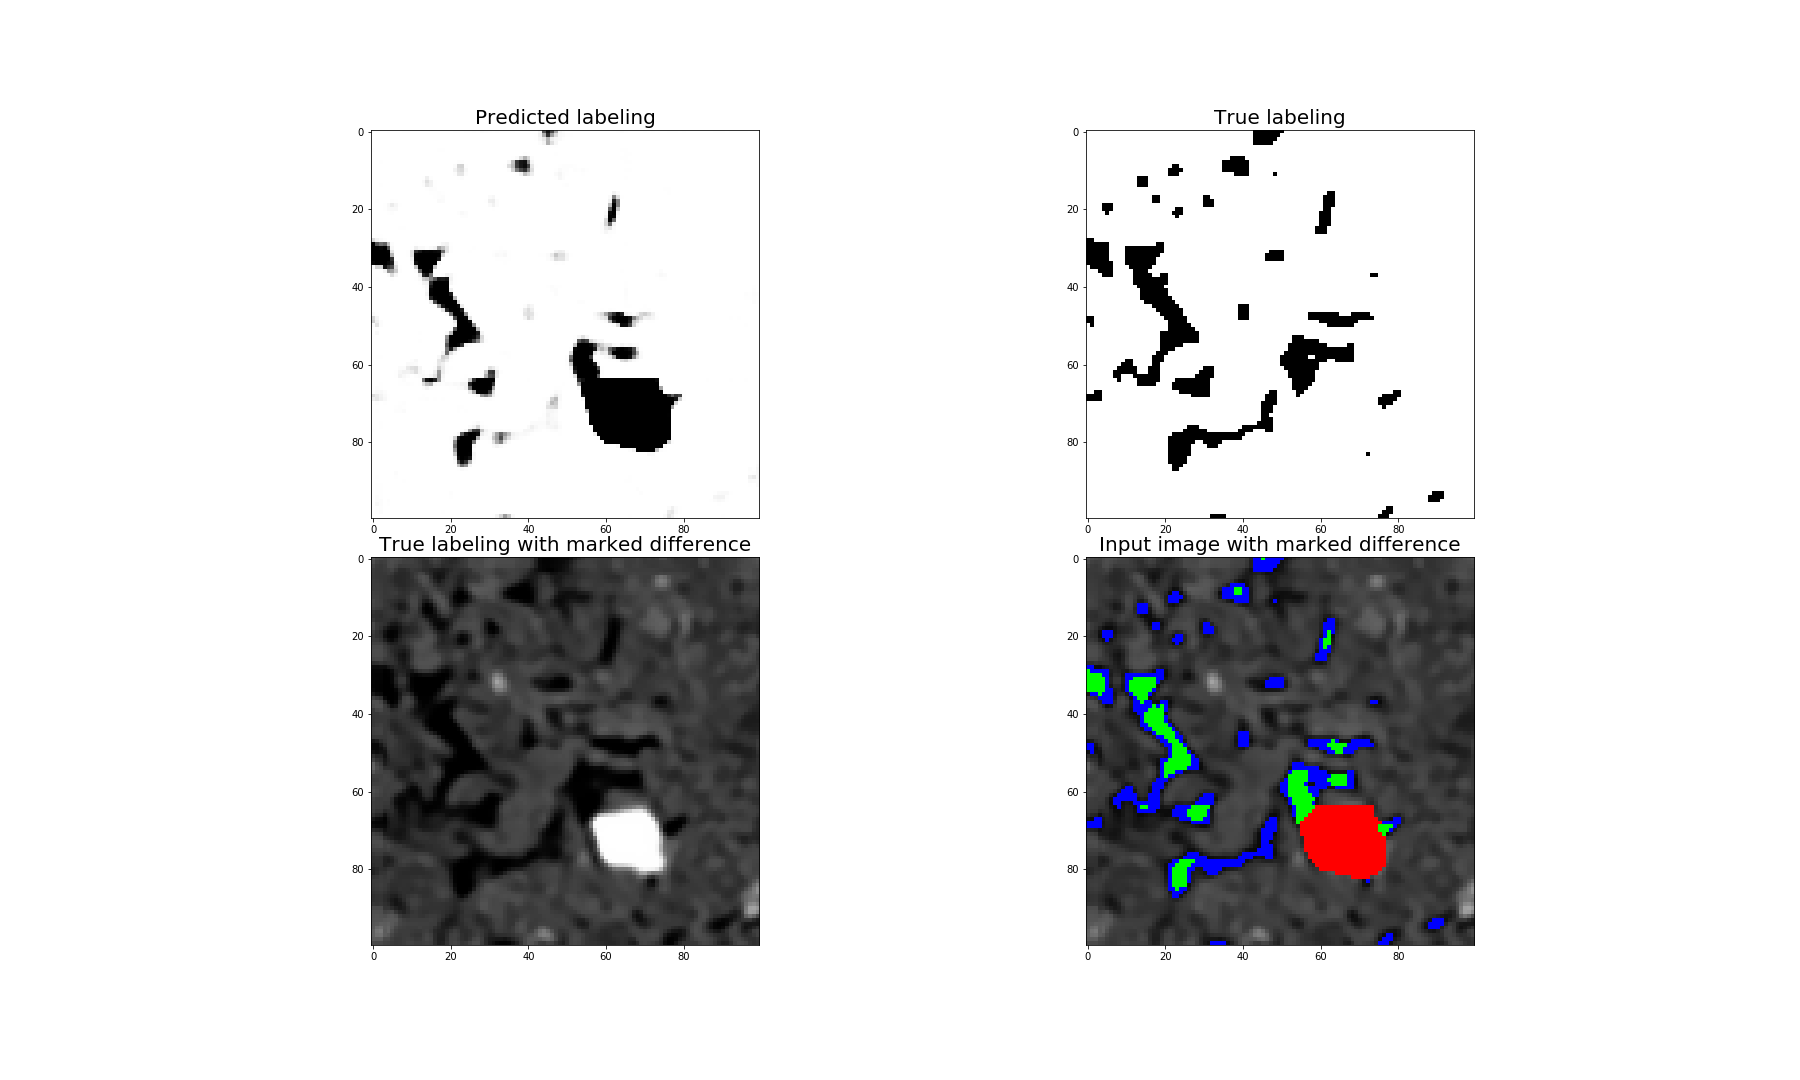
\includegraphics[width=1\linewidth]
			{data/predictions/carb96558/Urna_22jpg.png}
	}
	\caption{Model trained on carb96558 and predicts Urna22}
	\label{Results:visual_bright_cluster}
\end{figure}


\begin{figure}[h]
	\center{
		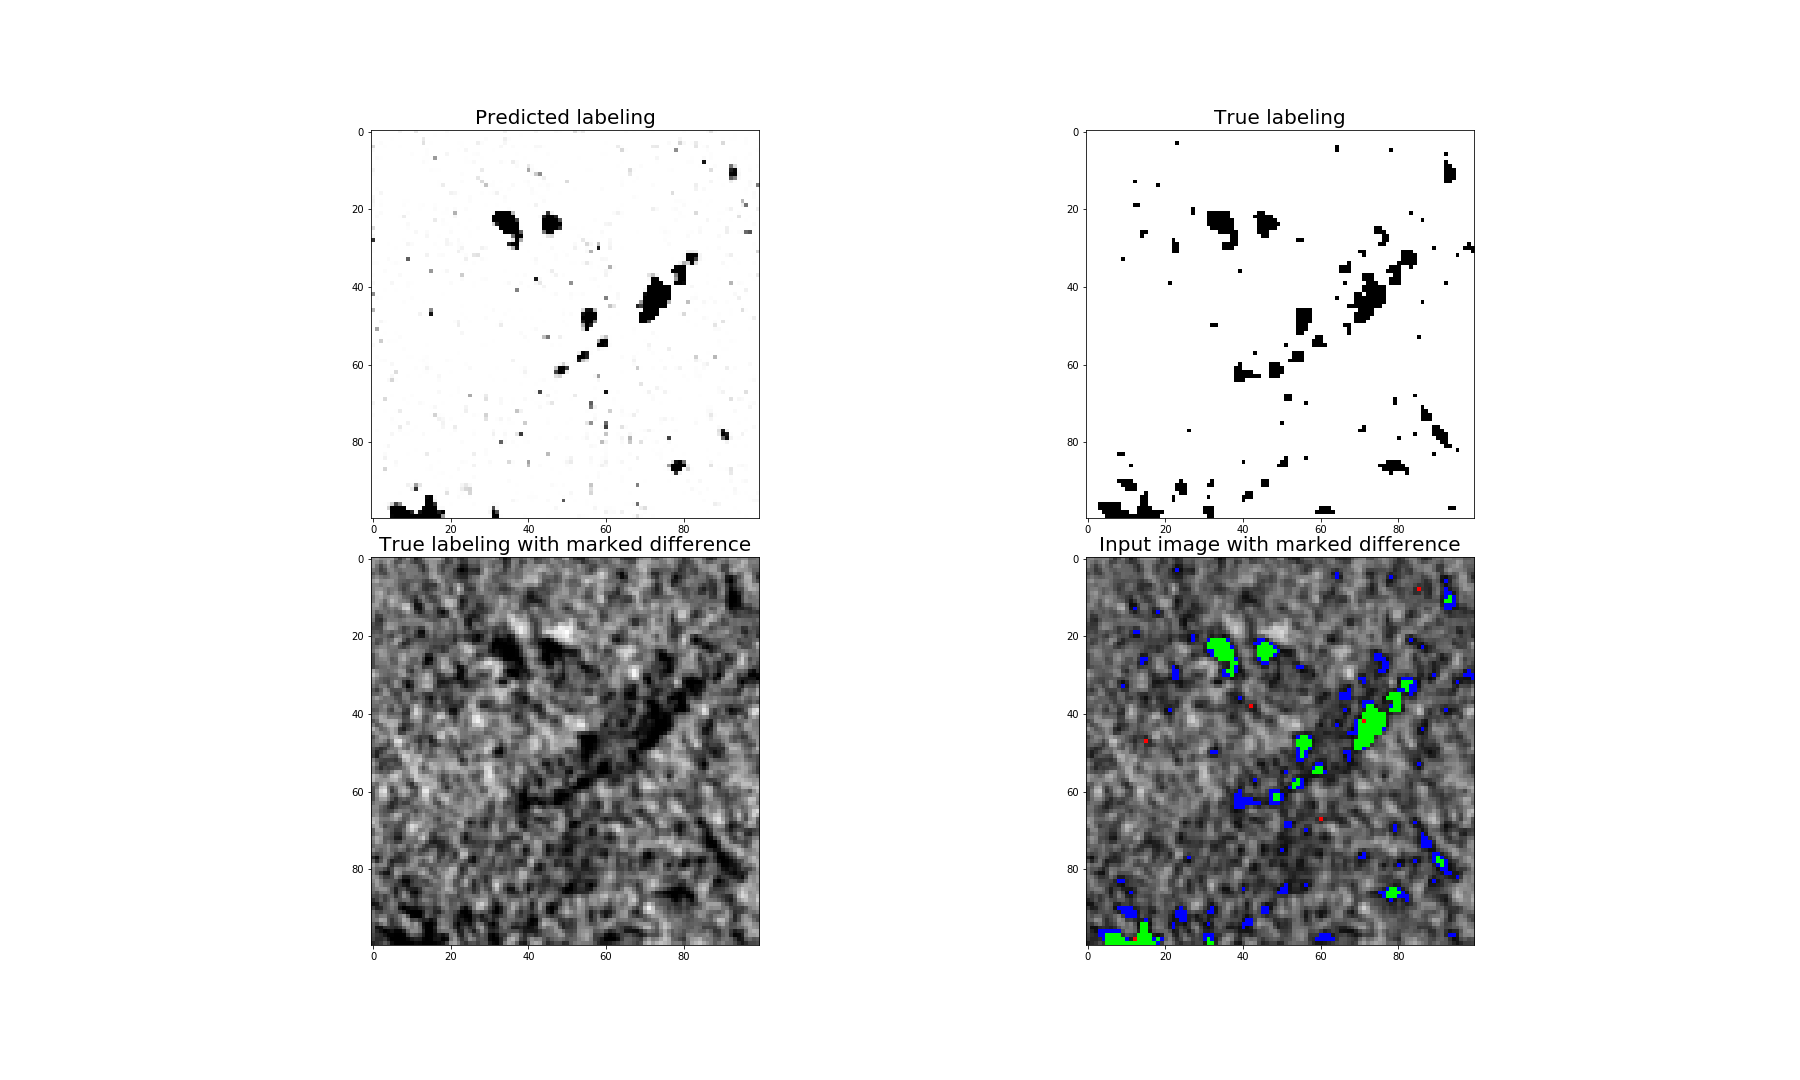
\includegraphics[width=1\linewidth]
			{data/predictions/carb96558/carbRNFjpg.png}
	}
	\caption{Model trained on carb96558 and predicts carbRNF, good prediction}
	\label{Results:visual_good_carbRNF}
\end{figure}

\begin{figure}[h]
	\center{
		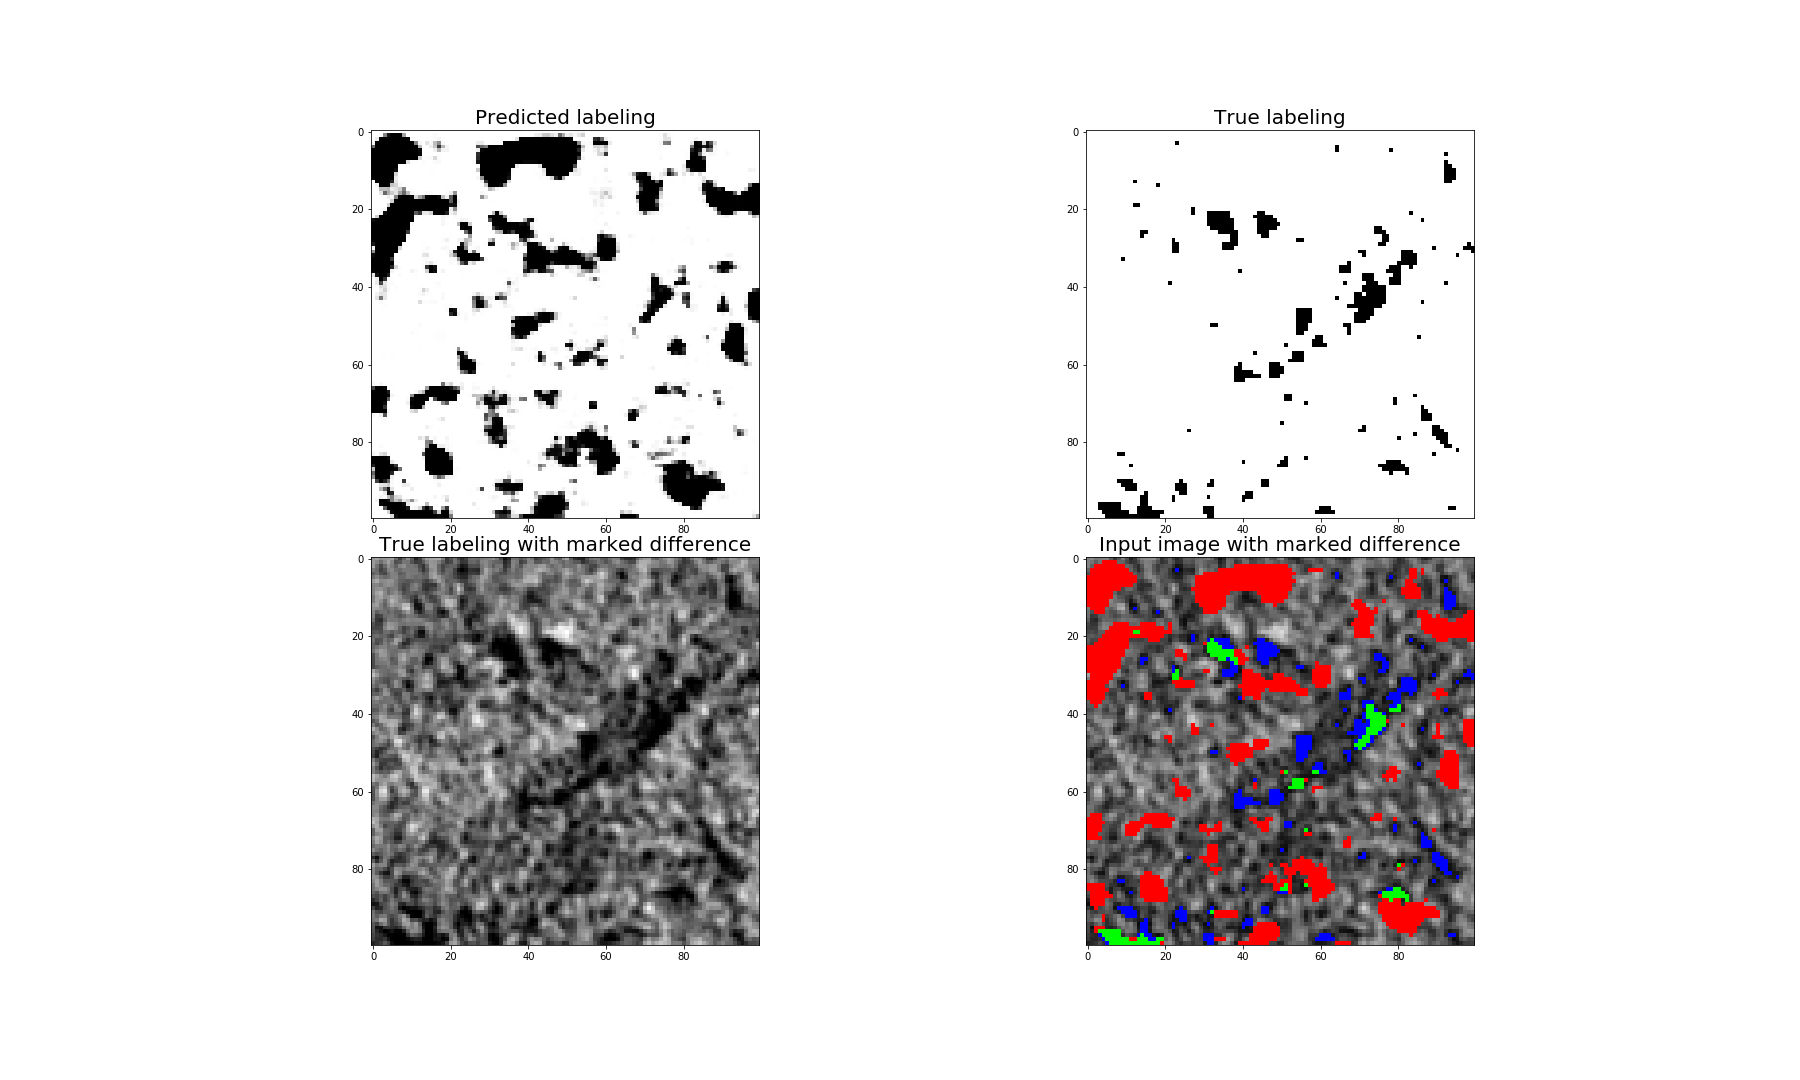
\includegraphics[width=1\linewidth]
			{data/predictions/SoilB-2/carbRNFjpg.png}
	}
	\caption{Model trained on SoilB-2 and predicts carbRNF, bad prediction}
	\label{Results:visual_bad_carbRNF}
\end{figure}

\begin{figure}[h]
	\center{
		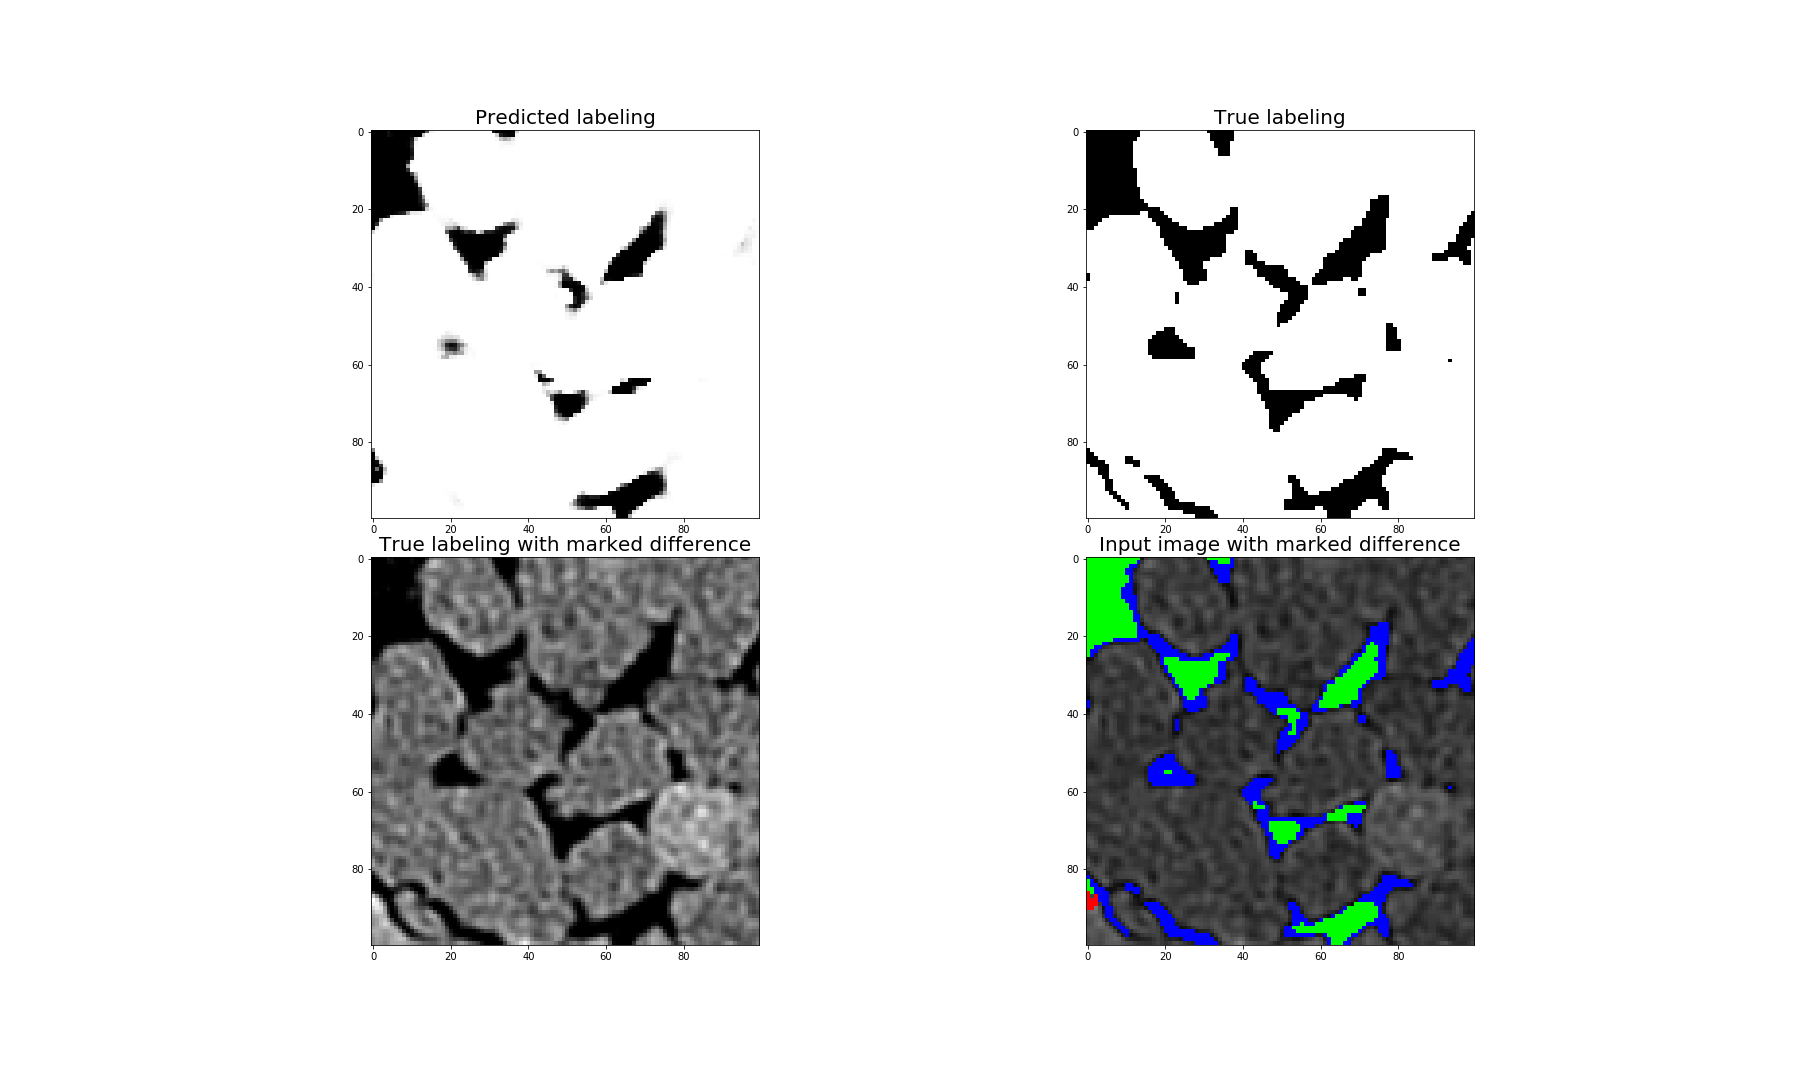
\includegraphics[width=1\linewidth]
			{data/predictions/carb96558_SoilB-2/Urna_34jpg.png}
	}
	\caption{Model trained on carb96558 and SoilB-2 and predicts Urna34, unconfident model}
	\label{Results:visual_unconfident}
\end{figure}

\subsection{Numerical segmentation results}

We create large table with measurements, so we could draw some conclusion. 

\begin{itemize}
	\item Specific models that trained on some stack type shows excelent perfomance on stacks from same type, but could do bad predictions on stacks from another type.
	\item Aggregate models show good perfomance on all stacks, so 
their outperform specific models in average, but lose on stacks with type that native for specific model.
\end{itemize}


\section{Discussion}
Overview of results and applicability of the results.

\section{Conclusion}
General conclusion and future work.

\section*{References}

\bibliography{mybibfile}

\end{document}